\section{Experiments}
\label{sec:exp}
We apply our research method experimentally on a large spatial-temporal dataset collected from IEEE dataport. By comparing the result with real events in Coronanet which records government responses to coronavirus, we evaluate the plausibility of the method. The result shows several points of interest in a specific time period and the details within each topic.
\subsection{Dataset Description and Experiment Setup}
{\bf Dataset}: 

The dataset we used is CORONAVIRUS (COVID-19) GEO-TAGGED TWEETS DATASET form IEEE DataPort. This dataset includes English tweets related to the epidemic from 2020 to 2022 around the world. Due to the tweets spreading policy. We can't access the
completed tweets content directly. The original data contains tweets ID and sentiment score calculated by
dataset publisher such as:
\begin{verbatim}
    ID                          SCORE
    12407280659839XXXXX         0.275
\end{verbatim} 

We use tweets ID to
request twitter API in batch and get completed information, including
content, UTC time, geographic location. All of these information are fully
imported into the server after splicing with sentiment score.  In this
process, we will transfer the longitude and latitude to the geometry, then we
can apply some spatial operator to handle them.

We use a transfer program named
Twarc to batch fetch tweets in the dataset. Twarc is a python package
that used to export tweets automatically.  The main principle is that Twarc
will make use of the registration information from twitter developer platform
and get the permission from Twitter. Then Twitter can monitor the whole
process of getting tweets. This way is completely legal and doesn't violate
the privacy protocols set by Twitter. But it also cause some issues. If the
tweets account is banned or the permission has been changed, we can't access
the content anymore. Normally Twitter doesn't send any warning message but
change the content of tweets to a prompt message. So some filtering process
is necessary to ensure that the data set is not contaminated with irrelevant
information. 

We collect data from March 2020 to March 2022. and store all of these data
to Elasticsearch with some batch programs, in order to facilitate subsequent steps to call on demand. 

{\bf Scope of research}:
COVID-19 related tweets contain many types of topic. To avoid noise, we narrow our research from multiple perspectives. According to some statistical conclusions of the epidemic, we choose the time period May 2020 to August 2021 when the epidemic is most concerned. Geographically, we choose the continental United States as the research target. Besides, we set a keywords list to filter tweets, so as to limit the influence of irrelevant topics as much as possible. (e.g. Posts about the city Corona instead of Coronavirus) All these search criterias are combined into one search request. 
The resulting sub-dataset will be used as the rearch object.

{\bf Preprocess}: 

The pre-processing process includes regex filtering, tokenization and tagging,
removal of stop words. Regex
filtering process is used to remove contents from which it is hard to obtain aluable information, such as URL, emoji, username, misspelled words. We also extract all hashtags from it.  

Tokenization and tag are important to our project. We use nltk package to
process the sentence in the tweets and decompose the content into single
words. Then we can filter for parts of speech and get more reasonable
results. 
\begin{figure}[h]
\centering
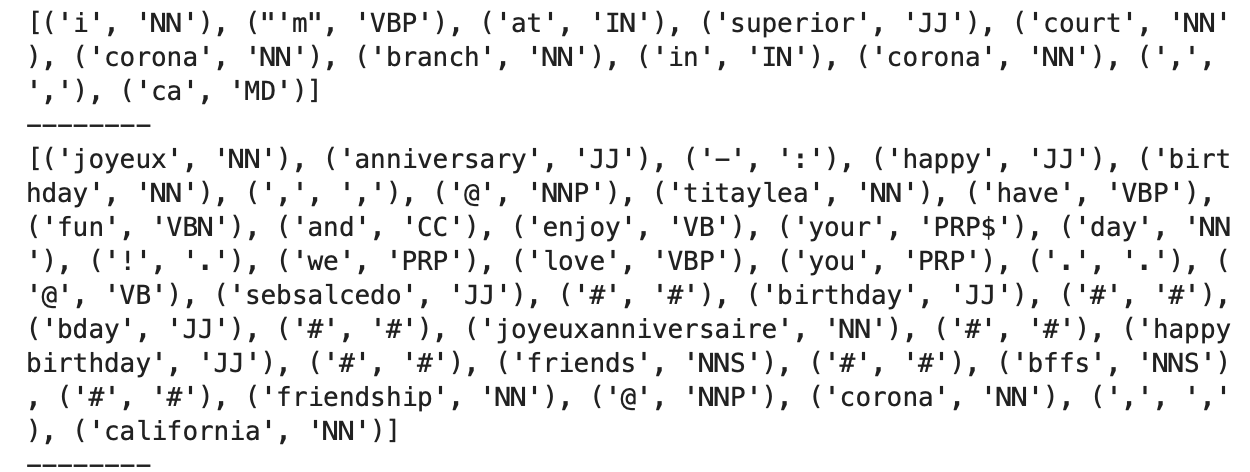
\includegraphics[width=0.5\textwidth]{imgs/tokenization.png}
\caption{Tokenization and tag}
\label{fig:Tokenization and tag}
\end{figure}
The purpose of removal of stopwords is to avoid distractions from common words
on the topic. The nltk package provide a library of stopwords and we can set
our own list of common words based on the theme. It's an important step to
get good performance of machine learning models and we can adjust it to fit
the current strategy we used.

{\bf Metrics}:

We use silhouette factor to evaluate the performance of clustering. For storyline generation, we based on rationality of the time series and topic keywords. 

{\bf Topic mining}:

To evaluate the quality of generated topics, we focus on both the content of the topic itself and the distribution of the topic. 


In the experiment, each topic consists of a series of related sentence vectors. We use high-frequency words in WordCloud to show the content of the topic. Besides, We also output one of the most representative sentences in each topic as supporting evidence. 

The distribution of clusters in the vector space is another indicator of the quality of the results. The projection of vectors in two-dimensional space can intuitively see the distribution of the cluster. In order to verify the temporal relevance of the topic we also use the time label of the topic vector as the third axis to generate a three-dimensional vector distribution map.

{\bf Comparison Models}: 

We propose a combination of lda and bert methods to produce high-quality sentence vectors. To verify the advantages of this approach, we output the clustering results using bert and LDA separately. We make a comprehensive assessment based on the quality of the topics and timelines generated by each method
\subsection{Results and Discussion}
\subsubsection{Evaluation of clustering}

 We adjust the number of clusters and weight ratio of the vector structure to get the best silhouette score. The quality of the generated storyline will also be a reference. For tweets dataset from May 2020 to August 2021, we found that silhouette score is maximized when the number of clusters is set to 18 and gamma is set to 9. We use this parameter pair for clustering in subsequent experiments.



\begin{table}[]
\begin{tabular}{ccccc}
\hline
\multicolumn{5}{c}{Silhouette score under different conditions}                                                                                                    \\ \hline
\multicolumn{1}{|c|}{conditions} &
  \multicolumn{1}{l|}{\textbf{gamma = 6}} &
  \multicolumn{1}{c|}{\textbf{gamma = 7}} &
  \multicolumn{1}{c|}{\textbf{gamma = 8}} &
  \multicolumn{1}{c|}{\textbf{gamma = 9}} \\ \hline
\multicolumn{1}{|c|}{\textbf{k = 16}} & \multicolumn{1}{c|}{0.003}  & \multicolumn{1}{c|}{0.028}  & \multicolumn{1}{c|}{0.025}  & \multicolumn{1}{c|}{-0.005}      \\ \hline
\multicolumn{1}{|c|}{\textbf{k = 18}} & \multicolumn{1}{c|}{0.021}  & \multicolumn{1}{c|}{-0.007} & \multicolumn{1}{c|}{0.017}  & \multicolumn{1}{c|}{{\ul 0.040}} \\ \hline
\multicolumn{1}{|c|}{\textbf{k = 20}} & \multicolumn{1}{c|}{0.015}  & \multicolumn{1}{c|}{-0.006} & \multicolumn{1}{c|}{0.008}  & \multicolumn{1}{c|}{0.032}       \\ \hline
\multicolumn{1}{|c|}{\textbf{k = 22}} & \multicolumn{1}{c|}{0.000}  & \multicolumn{1}{c|}{0.018}  & \multicolumn{1}{c|}{-0.008} & \multicolumn{1}{c|}{-0.006}      \\ \hline
\multicolumn{1}{|c|}{\textbf{k = 24}} & \multicolumn{1}{c|}{-0.009} & \multicolumn{1}{c|}{-0.008} & \multicolumn{1}{c|}{0.009}  & \multicolumn{1}{c|}{-0.013}      \\ \hline
\end{tabular}
\end{table}

\subsubsection{Topic content}
For each cluster we get, we focus on keywords and representative tweet within it. Fig~\ref{fig:wordcloud} shows an example. The wordcloud shows high frequencywords in current topic. As a supplement to the topic, we also obtained the central sentence of the cluster in each topic as the most representative tweet as:
\begin{verbatim}
    ID      sentences             time
    0       I got a vaccine...    2021-04-16 
    1       how covid impacts...  2020-09-29
    2       restaurant closed...  2020-11-27
    ...  
\end{verbatim} 
By these methods above, we show what people really care about in this topic.
\begin{figure}
\centering
{
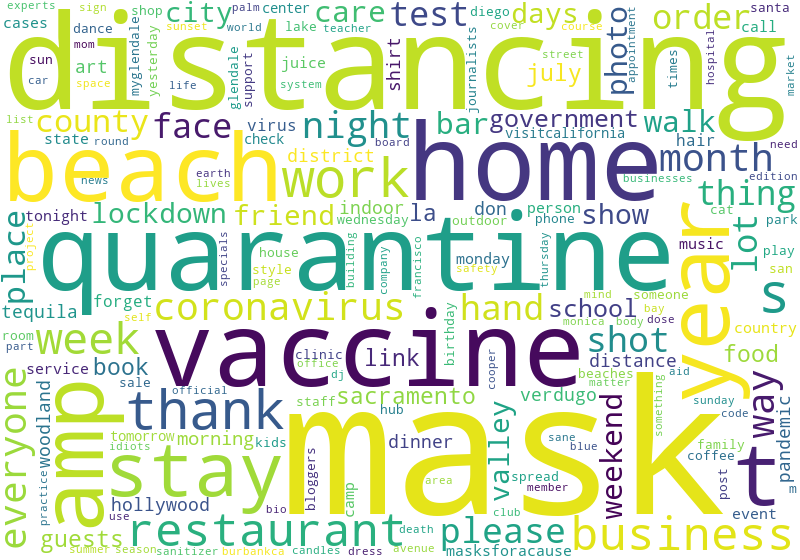
\includegraphics[width=0.4\textwidth]{imgs/lda_bert/Topic0_wordcloud.png}
\caption{wordcloud for one topic}
\label{fig:wordcloud}
}
\end{figure}


\subsubsection{Storyline}
Fig~\ref{fig:storyline for lda} shows a result of storyline from LDA-BERT.  

Each node in the graph represents a topic. From the label of nodes, we can get a list of high frequency words and published time. The number attached on the edges stand for a measure for correlation. Nodes with dark backgrounds are connected in series to form a storyline. The connection relationship between nodes reflects the connection between topics.

\begin{figure}[h]
\centering
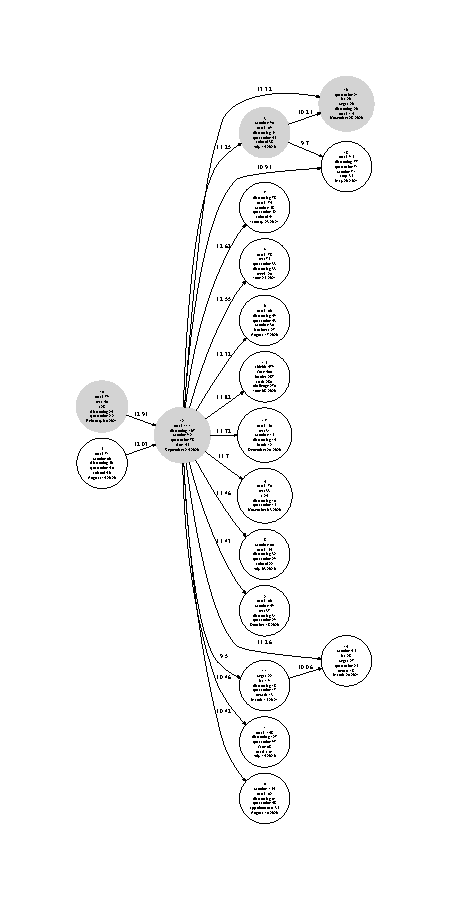
\includegraphics[width=0.5\textwidth]{imgs/lda_bert/storyline_lda_bert.gv.pdf}
\caption{slice of storyline for LDA-BERT}
\label{fig:storyline for lda_bert}
\end{figure}


\subsubsection{Model comparision}
For each method, we produce a 2D distribution graph to show the relevance of each cluster in terms of time and content. Fig~\ref{fig:2d_derivation for lda} shows a relatively scattered clustering results. However,in Fig~\ref{fig:storyline for lda} we can see that using lda alone result in too many topics mixed with noise. 

Fig~\ref{fig:2d_derivation for bert} shows poor clustering results that lots of clusters mixed together. It is difficult to reflect the inherent characteristics of each topic.

Fig~\ref{fig:2d_derivation for lda_bert} shows a compromised clustering effect. Some distinct clusters can be found at the edges of the graph. Meanwhile the topic generated from this method shows stronger noise immunity, refer to Fig~\ref{fig:storyline for lda_bert}

\begin{figure}
\centering
{
\includegraphics[width=0.4\textwidth]{imgs/lda/2d_vis.png}
\caption{2d derivation for LDA}
\label{fig:2d_derivation for lda}
}
\hspace{10pt}    %每张图片水平距离
{
\includegraphics[width=0.4\textwidth]{imgs/bert/2d_vis.png}
\caption{2d derivation for BERT}
\label{fig:2d_derivation for bert}
}
\hspace{10pt}
{
\includegraphics[width=0.4\textwidth]{imgs/lda_bert/2d_vis.png}
\caption{2d derivation for LDA-BERT}
\label{fig:2d_derivation for lda_bert}
}
\hspace{10pt}
\end{figure}
\begin{figure}[h]
\centering
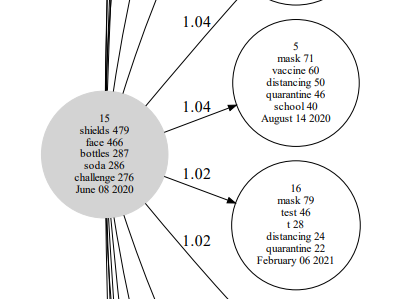
\includegraphics[width=0.5\textwidth]{imgs/lda/storyline.png}
\caption{slice of storyline for lda}
\label{fig:storyline for lda}
\end{figure}

\subsubsection{Derivation of topic}
Our framework also produce a 3D distribution graph for the topic to show the time correlation, refer to Fig~\ref{fig:3D distribution}, where vertical z-axis stand for time. We can find that some topics are time-sensitive, which may reflect a shift in people's attention.

\begin{figure}[h]
\centering
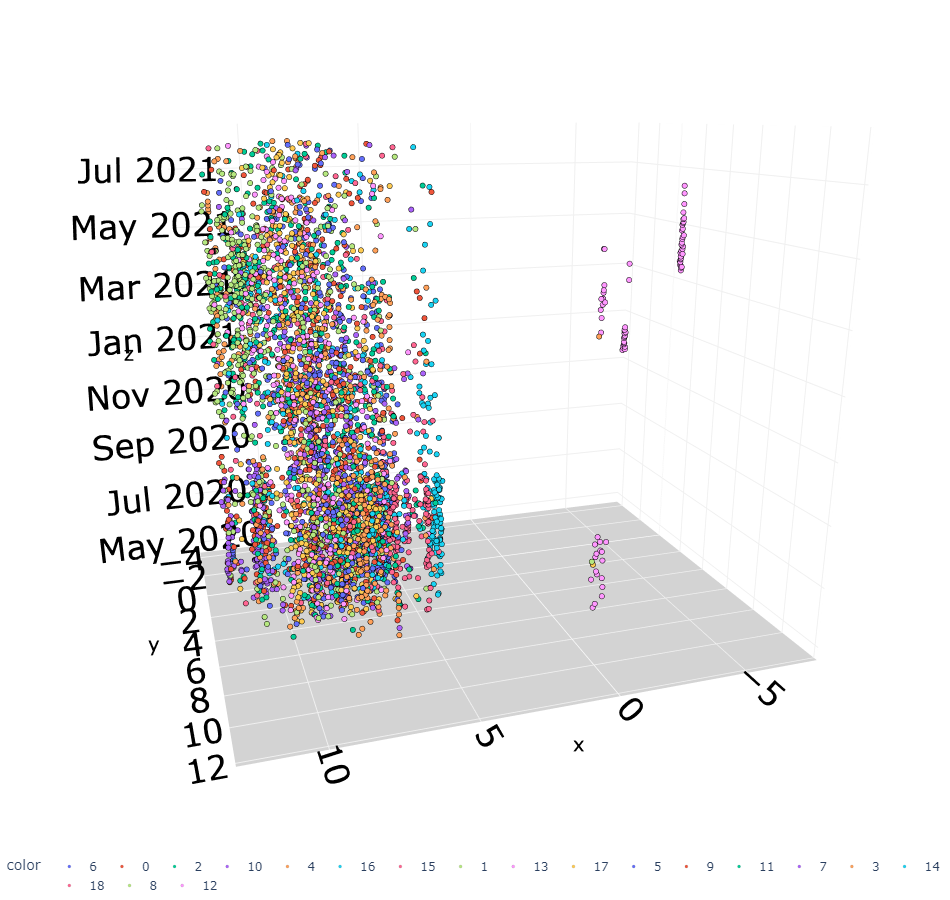
\includegraphics[width=0.5\textwidth]{imgs/lda_bert/3D_vis.png}
\caption{3D distribution graph}
\label{fig:3D distribution}
\end{figure}